\documentclass[12pt,a4paper]{article}
\usepackage[margin=2cm]{geometry}
\usepackage[T1]{fontenc}
\usepackage[utf8]{inputenc}
\usepackage{graphicx}
\usepackage{tikz}
\usetikzlibrary{arrows.meta, positioning}
\usepackage{setspace}
\emergencystretch=3em
\pagestyle{empty}

\begin{document}

\begin{center}
\vspace*{0.4cm}

\includegraphics[width=3.3cm]{assets/univo-logo.png}

\vspace{0.9cm}
{\LARGE\bfseries UNIVERSIDAD DE ORIENTE}

\vspace{0.35cm}
{\large FACULTAD DE INGENIER\'IA Y ARQUITECTURA}

\vspace{1.3cm}
{\large C\'ATEDRA:}

\vspace{0.2cm}
{\large Desarrollo de aplicaciones m\'oviles}

\vspace{1.1cm}
{\large CATEDR\'ATICO:}

\vspace{0.2cm}
{\large Fernando Alexis Blanco Gonzalez}

\vspace{1.1cm}
{\large ACTIVIDAD:}

\vspace{0.2cm}
{\large Creaci\'on del perfil de usuario}

\vspace{1.1cm}
{\large ESTUDIANTE}

\vspace{0.2cm}
{\large Anibal Josu\'e Campos Andrade - U20230770}

\vspace{0.45cm}
{\large Jueves 17 de septiembre, 2026}

\vspace{0.15cm}
{\large San Miguel, El Salvador}
\end{center}

\newpage
\noindent{\large\bfseries Resumen t\'ecnico: flujo de datos del perfil}

\vspace{0.5cm}

\noindent La pantalla de perfil (\texttt{app/(protected)/profile.tsx}) consume los datos del usuario autenticado a trav\'es del estado global de sesi\'on, siguiendo este flujo:

\begin{enumerate}
\item \textbf{Login:} desde \texttt{app/(public)/index.tsx} se invoca \texttt{AuthService.login()}, que realiza un \texttt{POST} a \texttt{/auth/login} y retorna \texttt{\{token, userResponse\}}.
\item \textbf{Persistencia:} \texttt{saveSession()} del \texttt{AuthContext} guarda el token y el usuario en \texttt{AsyncStorage} (\texttt{@auth\_token}, \texttt{@auth\_user}) y actualiza el estado global.
\item \textbf{Restauraci\'on:} al montar la aplicaci\'on, el \texttt{AuthProvider} recarga la sesi\'on desde \texttt{AsyncStorage} y expone \texttt{user} mediante el hook \texttt{useAuth()}.
\item \textbf{Renderizado:} en el perfil, \texttt{const \{user\} = useAuth()} provee el modelo \texttt{UserResponse} (\texttt{name}, \texttt{lastName}, \texttt{email}, \texttt{phone}, \texttt{image}, \texttt{roles}). Los inputs de nombre, correo y tel\'efono despliegan esos campos de forma reactiva con valores de respaldo ante nulos.
\item \textbf{Encabezado:} el avatar, nombre y rol provienen de \texttt{useDrawer()}, que deriva el perfil del mismo objeto \texttt{user} del contexto.
\item \textbf{Navegaci\'on:} el bot\'on de retroceso usa \texttt{router.canGoBack()} y, como respaldo, \texttt{router.replace()} hacia \texttt{/dashboard}, evitando la excepci\'on ``GO\_BACK not handled'' del drawer.
\end{enumerate}

\vspace{0.4cm}
\noindent{\bfseries Diagrama de flujo de datos}

\vspace{0.3cm}
\begin{center}
\resizebox{\textwidth}{!}{%
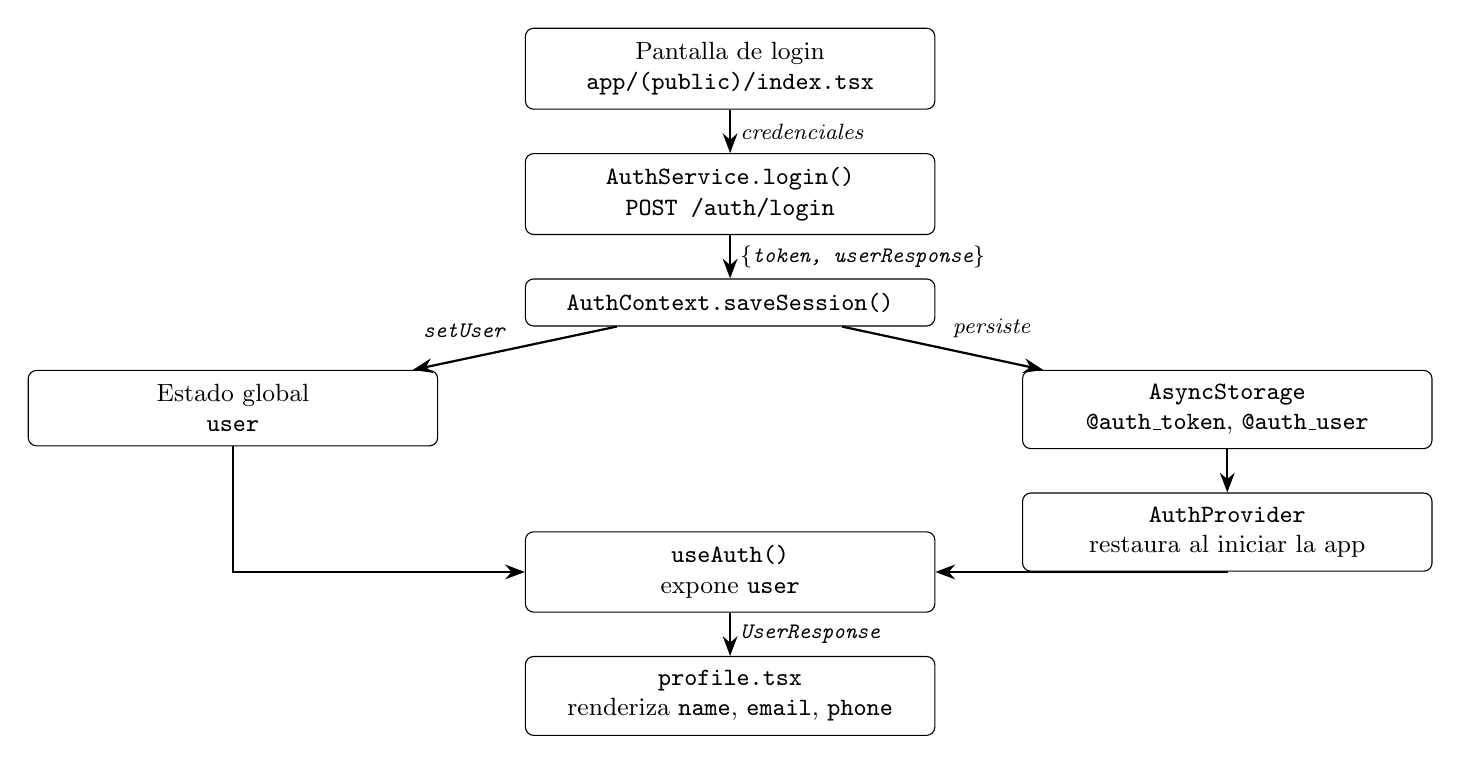
\begin{tikzpicture}[
    node distance=0.55cm and 1.1cm,
    box/.style={draw, rounded corners=3pt, align=center, inner sep=5pt,
                minimum width=5.2cm, font=\small},
    lbl/.style={font=\footnotesize\itshape},
    arr/.style={-{Stealth[length=2.5mm]}, thick},
  ]
  \node[box] (login) {Pantalla de login\\ \texttt{app/(public)/index.tsx}};
  \node[box, below=of login] (api) {\texttt{AuthService.login()}\\ \texttt{POST /auth/login}};
  \node[box, below=of api] (ctx) {\texttt{AuthContext.saveSession()}};
  \node[box, below left=of ctx] (state) {Estado global\\ \texttt{user}};
  \node[box, below right=of ctx] (storage) {\texttt{AsyncStorage}\\ \texttt{@auth\_token}, \texttt{@auth\_user}};
  \node[box, below=of storage] (provider) {\texttt{AuthProvider}\\ restaura al iniciar la app};
  \node[box, below=2.6cm of ctx] (hook) {\texttt{useAuth()}\\ expone \texttt{user}};
  \node[box, below=of hook] (ui) {\texttt{profile.tsx}\\ renderiza \texttt{name}, \texttt{email}, \texttt{phone}};

  \draw[arr] (login) -- node[lbl, right] {credenciales} (api);
  \draw[arr] (api) -- node[lbl, right] {\texttt{\{token, userResponse\}}} (ctx);
  \draw[arr] (ctx) -- node[lbl, above left] {\texttt{setUser}} (state);
  \draw[arr] (ctx) -- node[lbl, above right] {persiste} (storage);
  \draw[arr] (storage) -- (provider);
  \draw[arr] (state.south) |- (hook.west);
  \draw[arr] (provider.south) |- (hook.east);
  \draw[arr] (hook) -- node[lbl, right] {\texttt{UserResponse}} (ui);
\end{tikzpicture}}
\end{center}

\newpage
\noindent{\large\bfseries Evidencia de ejecuci\'on}

\vspace{0.5cm}

% Cuando tengas la captura, guardala como docs/perfil-usuario/assets/evidencia.png,
% descomenta la linea siguiente y elimina el recuadro placeholder:
% \noindent\includegraphics[width=\textwidth]{assets/evidencia.png}

\noindent\fbox{%
\begin{minipage}[c][0.72\textheight][c]{\dimexpr\textwidth-2\fboxsep-2\fboxrule}
\centering\large
[ESPACIO PARA CAPTURA DE PANTALLA COMPLETA]\\[0.6cm]
\normalsize La captura debe mostrar simult\'aneamente:\\[0.3cm]
$\bullet$ Emulador/dispositivo con la pantalla de Perfil\\
y los datos del usuario autenticado en los inputs\\[0.2cm]
$\bullet$ VS Code con \texttt{app/(protected)/profile.tsx} activo\\[0.2cm]
$\bullet$ Terminal integrada ejecutando Expo sin errores
\end{minipage}}

\end{document}
